\documentclass[tikz,border=5pt]{standalone}
\usepackage{amsmath,amssymb,fontspec,unicode-math}
\setmainfont{STIXTwoText-Regular.otf}
\setmathfont{STIXTwoMath-Regular.otf}
\usetikzlibrary{positioning,arrows.meta,calc,decorations.pathreplacing}
\definecolor{hmtgray}{gray}{0.3}
\definecolor{hmtblue}{gray}{0.15}
\definecolor{hmtgold}{gray}{0.3}
\definecolor{hmtgreen}{gray}{0.1}
\definecolor{hmtred}{gray}{0.25}
\definecolor{hmtlightblue}{gray}{0.92}
\definecolor{hmtlightgold}{gray}{0.83}
\definecolor{hmtlightgreen}{gray}{0.97}
\definecolor{hmtlightred}{gray}{0.73}
\begin{document}
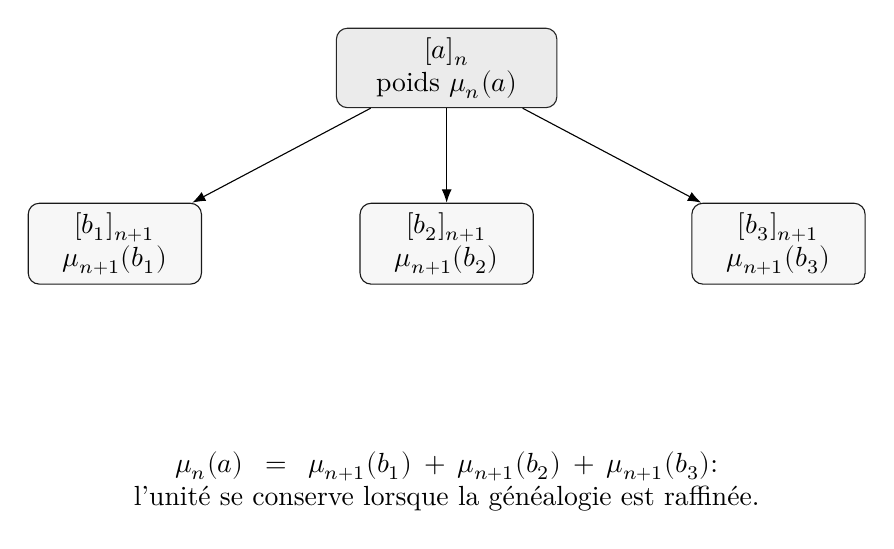
\begin{tikzpicture}[>=Latex,node distance=12mm and 17mm,
  box/.style={draw=hmtblue,rounded corners,fill=hmtlightblue,align=center,
              minimum width=28mm,minimum height=8mm},
  leaf/.style={draw=hmtgreen,rounded corners,fill=hmtlightgreen,align=center,
               minimum width=22mm,minimum height=7mm}]
\node[box] (a) {$[a]_n$\\poids $\mu_n(a)$};
\node[leaf,below left=of a] (b1) {$[b_1]_{n+1}$\\$\mu_{n+1}(b_1)$};
\node[leaf,below=of a] (b2) {$[b_2]_{n+1}$\\$\mu_{n+1}(b_2)$};
\node[leaf,below right=of a] (b3) {$[b_3]_{n+1}$\\$\mu_{n+1}(b_3)$};
\draw[->] (a)--(b1); \draw[->] (a)--(b2); \draw[->] (a)--(b3);
\node[below=20mm of b2,align=center,text width=.78\textwidth] (eq)
 {$\mu_n(a)=\mu_{n+1}(b_1)+\mu_{n+1}(b_2)+\mu_{n+1}(b_3)$:\\
  l’unité se conserve lorsque la généalogie est raffinée.};
\end{tikzpicture}
\end{document}

